\definecolor{amministratore}{RGB}{51,102,204}
\definecolor{analista}{RGB}{255,153,0}
\definecolor{progettista}{RGB}{153,0,153}
\definecolor{programmatore}{RGB}{7,55,99}
\definecolor{responsabile}{RGB}{220,57,18}
\definecolor{verificatore}{RGB}{16,150,24}

\section{Prospetto economico}

In questa sezione è presentato il prospetto economico del progetto \ProjectName{}, suddiviso per fasi. Per ogni fase sono indicate le ore preventivate per ogni ruolo impiegato.
Il costo è calcolato utilizzando i dati della tabella al paragrafo \ref{tabellacostiruolo}.

\subsection{Analisi}

A scopo di trasparenza viene redatto il prospetto economico riguardante la fase di Analisi dei requisiti, ma si precisa che le ore spese in questa fase sono a carico del fornitore e non del proponente.

\begin{table}[H]
	\centering
	\begin{tabular}{ l c c }
	\textbf{Ruolo} & \textbf{Ore} & \textbf{Costo} \\
	\hline
		Amministratore & 30 & 600 € \\
	Analista & 58 & 1450 € \\
	Progettista & 9 & 198 € \\
	Programmatore & 0 & 0 € \\
	Responsabile & 14 & 420 € \\
	Verificatore & 31 & 465 € \\
\hline
	Totale & 142 & 3133 € \\
\hline

	\end{tabular}
	\caption{Ore e costo per ruolo, fase di Analisi}
	\end{table}

I seguenti grafici mostrano il peso orario e di costo di ogni ruolo in questa fase.

\begin{figure}[H]
\begin{tikzpicture}

	\pie[text=legend, color={amministratore, analista, progettista, programmatore, responsabile, verificatore}]{21.1/Amministratore, 40.8/Analista, 6.3/Progettista, ./Programmatore, 9.9/Responsabile, 21.8/Verificatore}


\end{tikzpicture}
\caption{Ore per ruolo, fase di Analisi}
\end{figure}

\begin{figure}[H]
\begin{tikzpicture}

	\pie[text=legend, color={amministratore, analista, progettista, programmatore, responsabile, verificatore}]{19.2/Amministratore, 46.3/Analista, 6.3/Progettista, ./Programmatore, 13.4/Responsabile, 14.8/Verificatore}


\end{tikzpicture}
\caption{Costo per ruolo, fase di Analisi}
\end{figure}

\subsection{Progettazione architetturale}

Nella fase di Progettazione architetturale le ore per ogni ruolo sono state cosi suddivise:

\begin{table}[H]
	\centering
	\begin{tabular}{ l c c }
	\textbf{Ruolo} & \textbf{Ore} & \textbf{Costo} \\
	\hline
	
			Amministratore & 58 & 1160 € \\
	Analista & 22 & 550 € \\
	Progettista & 112 & 2464 € \\
	Programmatore & 0 & 0 € \\
	Responsabile & 27 & 810 € \\
	Verificatore & 74 & 1110 € \\
\hline
	Totale & 293 & 6094 € \\
\hline

	
	\end{tabular}
	\caption{Ore e costo per ruolo, fase di Progettazione architetturale}
	\end{table}
	
I seguenti grafici mostrano il peso orario e di costo di ogni ruolo in questa fase.

\begin{figure}[H]
\begin{tikzpicture}

	\pie[sum=auto, text=legend]{48/Amministratore, 24/Analista, 70/Progettista, 19.0/Responsabile, 42/Verificatore}


\end{tikzpicture}
\caption{Ore per ruolo, fase di Progettazione architetturale}
\end{figure}

\begin{figure}[H]
\begin{tikzpicture}

	\pie[text=legend, color={amministratore, analista, progettista, programmatore, responsabile, verificatore}]{32.9/Amministratore, 9.2/Analista, 39.6/Progettista, ./Programmatore, 8.7/Responsabile, 9.6/Verificatore}


\end{tikzpicture}
\caption{Costo per ruolo, fase di Progettazione architetturale}
\end{figure}


%\begin{figure}[H]
%\centering
%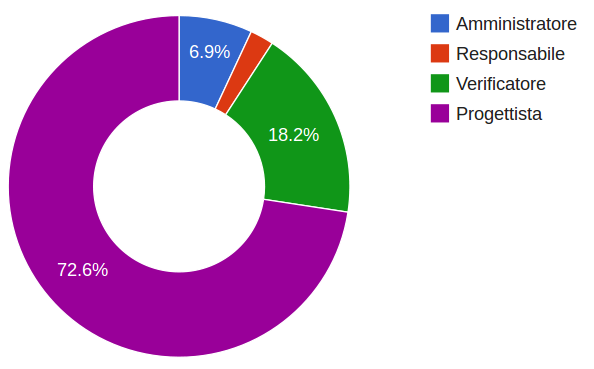
\includegraphics[scale=0.4]{5-2-2.png}
%\caption{Costo per ruolo, fase di Progettazione architetturale\label{fig:nome}}
%\end{figure}

\subsection{Progettazione di dettaglio e codifica}

Nella fase di Progettazione di dettaglio e codifica le ore per ogni ruolo sono state cosi suddivise:

\begin{table}[H]
	\centering
	\begin{tabular}{ l c c }
	\textbf{Ruolo} & \textbf{Ore} & \textbf{Costo} \\
	\hline
	
			Amministratore & 42 & 840 € \\
	Analista & 8 & 200 € \\
	Progettista & 66 & 1452 € \\
	Programmatore & 126 & 1890 € \\
	Responsabile & 4 & 120 € \\
	Verificatore & 54 & 810 € \\
\hline
	Totale & 300 & 5312 € \\
\hline

	
	\end{tabular}
	\caption{Ore e costo per ruolo, fase di Progettazione di dettaglio e codifica}
	\end{table}

I seguenti grafici mostrano il peso orario e di costo di ogni ruolo in questa fase.

\begin{figure}[H]
\begin{tikzpicture}

	\pie[sum=auto, text=legend]{38/Amministratore, 8/Analista, 120/Progettista, 132/Programmatore, ./Responsabile, 90/Verificatore}


\end{tikzpicture}
\caption{Ore per ruolo, fase di Progettazione di dettaglio e codifica}
\end{figure}

\begin{figure}[H]
\begin{tikzpicture}

	\pie[text=legend, color={amministratore, analista, progettista, programmatore, responsabile, verificatore}]{16.4/Amministratore, 3.8/Analista, 27.6/Progettista, 36.0/Programmatore, 2.3/Responsabile, 14.0/Verificatore}


\end{tikzpicture}
\caption{Costo per ruolo, fase di Progettazione di dettaglio e codifica}
\end{figure}

\subsection{Validazione}

Nella fase di Validazione le ore per ogni ruolo sono state cosi suddivise:

\begin{table}[H]
	\centering
	\begin{tabular}{ l c c }
	\textbf{Ruolo} & \textbf{Ore} & \textbf{Costo} \\
	
			Amministratore & 16 & 320 € \\
	Analista & 0 & 0 € \\
	Progettista & 8 & 176 € \\
	Programmatore & 0 & 0 € \\
	Responsabile & 8 & 240 € \\
	Verificatore & 98 & 1470 € \\
\hline
	Totale & 130 & 2206 € \\
\hline

	
	\end{tabular}
	\caption{Ore e costo per ruolo, fase di Validazione}
	\end{table}

I seguenti grafici mostrano il peso orario e di costo di ogni ruolo in questa fase.

\begin{figure}[H]
\begin{tikzpicture}

	\pie[sum=auto, text=legend]{30/Amministratore, ./Analista, ./Progettista, ./Programmatore, ./Responsabile, 110/Verificatore}


\end{tikzpicture}\caption{Ore per ruolo, fase di Validazione}
\end{figure}

\begin{figure}[H]
\begin{tikzpicture}

	\pie[text=legend, color={amministratore, analista, progettista, programmatore, responsabile, verificatore}]{14.5/Amministratore, ./Analista, 8.0/Progettista, ./Programmatore, 10.9/Responsabile, 66.6/Verificatore}


\end{tikzpicture}
\caption{Costo per ruolo, fase di Validazione}
\end{figure}

\subsection{Totale}

In totale le ore per ogni ruolo sono state cosi suddivise:

\begin{table}[H]
	\centering
	\begin{tabular}{ l c c }
	\textbf{Ruolo} & \textbf{Ore} & \textbf{Costo} \\
	\hline
	
			Amministratore & 102 & 2040 € \\
	Analista & 30 & 750 € \\
	Progettista & 184 & 4048 € \\
	Programmatore & 126 & 1890 € \\
	Responsabile & 35 & 1050 € \\
	Verificatore & 224 & 3360 € \\
\hline
	Totale & 701 & 13138 € \\
\hline

	
	\end{tabular}
	\caption{Ore e costo per ruolo, riassunto progetto}
	\end{table}

I seguenti grafici mostrano il peso orario e di costo di ogni ruolo durante tutto lo svolgimento del progetto, esclusa la fase di Analisi dei requisiti.

\begin{figure}[H]
\centering
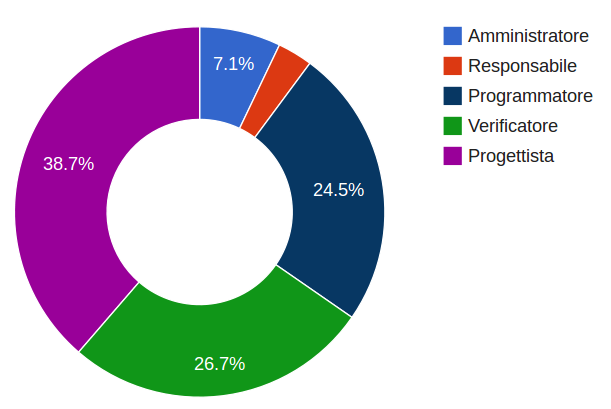
\includegraphics[scale=0.35]{5-5-1.png}
\caption{Ore per ruolo\label{fig:nome}}
\end{figure}

\begin{figure}[H]
\centering
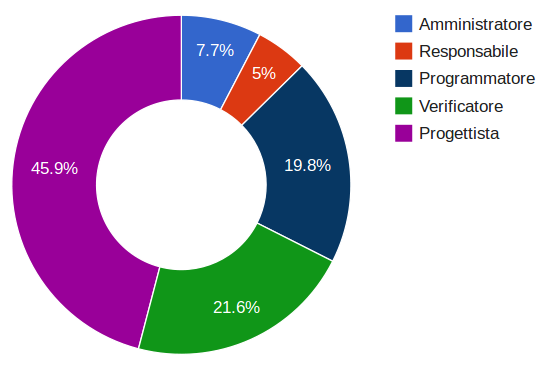
\includegraphics[scale=0.4]{5-5-2.png}
\caption{Costo per ruolo\label{fig:nome}}
\end{figure}
